\section{Available Expressions dan Global CSE}

Analisis \compiler{Available Expressions} adalah masalah \textbf{Forward} dengan meet operator \textbf{Intersection} ($\cap$). Analisis ini menentukan apakah sebuah perhitungan ekspresi sudah pernah dilakukan sebelumnya di semua jalur eksekusi yang memungkinkan.

\subsection{Persamaan Aliran Data (Intersection)}
Berbeda dengan Reaching Defs yang menggunakan Union, analisis ini menggunakan irisan karena sebuah ekspresi harus tersedia di \textbf{semua} jalur pendahulu:
\begin{enumerate}
    \item \textbf{Meet Operation}: $IN[B] = \bigcap_{P \in Pred(B)} OUT[P]$.
    \item \textbf{Transfer Function}: $OUT[B] = e\_gen[B] \cup (IN[B] - e\_kill[B])$.
\end{enumerate}

\subsection{Langkah Global CSE}
Global Common Subexpression Elimination menggunakan informasi ini untuk:
\begin{enumerate}
    \item Menemukan ekspresi $x + y$ yang \textit{available} di awal blok $B$.
    \item Melacak mundur ke titik-titik definisi ekspresi tersebut.
    \item Mengganti perhitungan di titik-titik tersebut dengan variabel temporary $t$.
    \item Mengganti penulisan ekspresi di blok $B$ dengan pembacaan dari variabel $t$.
\end{enumerate}

\begin{figure}[!htbp]
    \centering
    \adjustbox{max width=0.8\textwidth,center}{%
    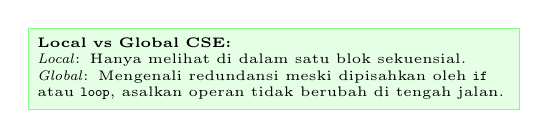
\begin{tikzpicture}[
        rect/.style={rectangle, draw=green!50, fill=green!10, text width=6cm, font=\tiny}
    ]
    \node[rect] (cse) {
        \textbf{Local vs Global CSE:}\\
        \textit{Local}: Hanya melihat di dalam satu blok sekuensial.\\
        \textit{Global}: Mengenali redundansi meski dipisahkan oleh \texttt{if} atau \texttt{loop}, asalkan operan tidak berubah di tengah jalan.
    };
    \end{tikzpicture}%
    }
    \caption{Perbandingan Ruang Lingkup CSE}
\end{figure}
